\section{Scaling factors for Primakoff, nuclear coherent, and nuclear incoherent cross sections  \label{sec:SigmaScaling}}
Fig.~\ref{fig:leaddndt} shows $^{208}$Pb data from the PrimEx experiment \cite{Larin:2010kq}.   NPP will run on the same target and the same approximate incident beam energy, $\approx 6$ GeV, as PrimEx.   Using known analytical forms for processes shown in the figure, known photo-nuclear cross sections, and estimates for nuclear attenuation from the PrimEx $^{208}$Pb analysis, numerical factors can be calculated  to scale the Primakoff, nuclear coherent and nuclear incoherent cross sections seen in PrimEx to the conditions for NPP. 
The modeling presented here does not take into account differing momentum transfers for $\gamma A \rightarrow A \pi^0 \pi^0$ (NPP) versus  $\gamma A \rightarrow A \pi^0 $ (PrimEx), which  has an important effect on the shape of the cross section distributions as a function of t (or $\theta$), primarily through the strong and electromagnetic form factors.    

 \subsection{Scale factor for the Primakoff cross section}
The standard equation for Primakoff $\pi^0$ production is given by: 

$$ { d^2 \sigma_{PrimEx} \over d \Omega } = \Gamma_{\pi^0 \rightarrow \gamma \gamma} { 8 \alpha Z^2 \over M^3_{\pi} }
{ \beta^3 E_\gamma^4 \over Q^4 } F^2_{EM}(Q^2) sin^2 \theta   $$ 

where $\Gamma_{\pi^0 \rightarrow \gamma \gamma} = 7.7$ eV is the $\pi^0$ radiative width.  The cross section for Primakoff $\pi \pi$ production with $P_{\gamma}=0$ is given by: 

$$ {d^2 \sigma_{NPP} \over d \Omega_{\pi \pi} dM_{\pi \pi} } = {2 \alpha Z^2 \over \pi^2} 
{E_\gamma^4 \beta^2 \over M_{\pi \pi} } {sin^2 \theta \over Q^4 } F^2_{EM}(Q^2) 
 \sigma( \gamma \gamma \rightarrow \pi \pi) $$

The equation can be reorganized so that its structure is similar to the standard Primakoff equation: 

$$ {d^2 \sigma_{NPP} \over d \Omega_{\pi \pi} } \approx
\Big[ {1 \over 4 \pi^2 }  {M^2_{\pi \pi} \over \beta }  \sigma( \gamma \gamma \rightarrow \pi \pi) \Delta M_{\pi \pi} \Big]  { 8 \alpha Z^2 \over M^3_{\pi \pi} }
{ \beta^3 E_\gamma^4 \over Q^4 } F^2_{EM}(Q^2) sin^2 \theta  $$

$$ {d^2 \sigma_{NPP} \over d \Omega_{\pi \pi} } \approx
\Gamma_{\pi^0 \pi^0 \rightarrow \gamma \gamma}  { 8 \alpha Z^2 \over M^3_{\pi \pi} }
{ \beta^3 E_\gamma^4 \over Q^4 } F^2_{EM}(Q^2) sin^2 \theta  $$

where  $\Gamma_{\pi^0 \pi^0 \rightarrow \gamma \gamma}$ is the effective radiative width for $\pi^0 \pi^0 \rightarrow \gamma \gamma$, 

$$ \Gamma_{\pi^0 \pi^0 \rightarrow \gamma \gamma} =\Big[ {1 \over 4 \pi^2 }  {M^2_{\pi \pi} \over \beta }  \sigma( \gamma \gamma \rightarrow \pi \pi) \Delta M_{\pi \pi} \Big] $$

Taking $M_{\pi \pi} \approx 0.4$ GeV, $\Delta M_{\pi \pi}\approx 0.4$ GeV, and $\sigma ( \gamma \gamma \rightarrow \pi^0 \pi^0) \approx 10$ nb gives, 

$$\Gamma_{\pi^0 \pi^0 \rightarrow \gamma \gamma} \approx 42\ eV$$

The ratio of Primakoff $\pi^0 \pi^0$ production in width $\Delta M_{\pi \pi}$  to Primakoff $\pi^0$ production is given by, 

$$  {d^2\sigma_{NPP} \over d\Omega dM_{\pi \pi}} \Delta M_{\pi \pi} \Big/ { d\sigma_{PrimEx} \over d\Omega} 
\approx 
\Big(\Gamma_{\pi^0 \pi^0 \rightarrow \gamma \gamma} 
\Big/ \Gamma_{\gamma \gamma} \Big)
\times \Big( M_\pi \Big/ 
M_{\pi \pi}\Big)^3
\approx 0.2$$

 \subsection{Scale factor for the nuclear coherent cross section}

The nuclear coherent cross section for  $\pi^0$ photo-production is given by: 

$$ {d\sigma_{\gamma A \rightarrow A  \pi^0 } \over dt } \approx \eta A^2 { d\sigma_{\gamma N \rightarrow N \pi^0 } \over dt } F^2(t) $$

where $\eta$ is the nuclear absorption factor for $\pi^0$ production, A is the atomic mass number, $d\sigma_{\gamma N \rightarrow N\pi^0 } / dt$ is the $\pi^0$ photo-production cross section on the nucleon, and $F(t)$ is the nuclear matter formfactor.  The nuclear coherent cross section for  $\pi^0 \pi^0$ photo-production has a similar form: 

$$ {d\sigma_{\gamma A \rightarrow A  \pi^0 \pi^0} \over dt } \approx  \eta^2 A^2 { d^2 \sigma_{\gamma N \rightarrow N \pi^0 \pi^0} \over dt dM_{\pi \pi}}\Delta M_{\pi \pi} F^2(t) $$

where $d^2\sigma_{\gamma \rightarrow N\pi^0 \pi^0} / dt dM_{\pi \pi}$ is the $\pi^0 \pi^0$ photo-production cross section on the nucleon.
  In the near threshold region the dominant channel for $\pi^0 \pi^0$ photo-production is the f$_0(500)$.    Photo-production cross sections for f$_0(500)$ have been measured in 
  $\gamma p \rightarrow \pi^+ \pi^-$ at 3.6-3.8 GeV \cite{Battaglieri:2009aa}.   The s-wave t and $M_{\pi^+ \pi^-}$ distributions are shown in Fig. \ref{f0_500}, the former at M$_{\pi \pi}=0.4$ GeV, and the latter at $t=0.5 GeV^2$.  Note that  
  $d\sigma^2 / dt dM_{\pi^+ \pi^-}$ is relatively flat versus M$_{\pi \pi}$ in the threshold region. The relevant cross section for this analysis is $d\sigma^2 / dt dM_{\pi^+ \pi^-} \approx 1.0 \mu b/GeV^3$ at $t\rightarrow 0$, multiplied by an isospin factor of 1/2 for the f$_0(500)$ branching fraction to $\pi^0 \pi^0$.   This gives $d \sigma_{\gamma N \rightarrow N \pi^0 \pi^0} / dt dM_{\pi \pi} \approx 0.5 \mu b / GeV^2 $. The cross section for  $\gamma p \rightarrow  p \pi^0$ at 6 GeV has been measured at SLAC \cite{Anderson:1971}, with cross sections shown in Fig. \ref{SLAC}:   $d\sigma / dt \approx 1.5 \mu b/GeV^2$ at $t \rightarrow 0$.   Estimates from the PrimEX $^{208}$Pb analysis give $\eta \approx 0.55$.  Using $\Delta M_{\pi \pi} = 0.4$ GeV, the ratio of  $\pi^0 \pi^0$ nuclear coherent photo-production in width  $\Delta M_{\pi \pi}$  to $\pi^0$ nuclear coherent photo-production is given by: 

$$  {d\sigma_{\gamma A \rightarrow A \pi^0 \pi^0} \over dt}  \Big/ { d\sigma_{\gamma A \rightarrow A \pi^0} \over dt}  \approx \eta 
 {d^2\sigma_{\gamma N \rightarrow N \pi^0 \pi^0} \over dt dM_{\pi \pi} } \Delta M_{\pi \pi} \Big/ { d\sigma_{\gamma N \rightarrow N \pi^0} \over dt} \approx 0.07 $$

\subsection{Scale factor for the nuclear incoherent cross section}

The nuclear incoherent cross section for  $\pi^0$ photo-production is given by: 

$$ {d\sigma_{\gamma A \rightarrow   \pi^0 } \over dt } \approx \eta A \Big(1 -G(t) \Big){ d\sigma_{\gamma N \rightarrow N \pi^0 } \over dt } F^2(t) $$

and the nuclear incoherent cross section for  $\pi^0 \pi^0$ photo-production has a similar form: 

$$ {d\sigma_{\gamma A \rightarrow   \pi^0 \pi^0 } \over dt } \approx \eta^2 A \Big(1 -G(t) \Big){ d^2\sigma_{\gamma N \rightarrow N \pi^0 \pi^0 } \over dt dM_{\pi \pi}} \Delta M_{\pi \pi} F^2(t) $$

where G(t) is a Pauli suppression factor, with G(0)=1, and $G(t)\rightarrow 0$ for $t> k_F$ where $k_F$ is the nuclear Fermi momentum.   The nucleon photo-production cross sections are identical to those used in the estimation of the nuclear coherent cross section.    The ratio of  $\pi^0 \pi^0$ nuclear incoherent photo-production in  width $\Delta M_{\pi \pi}$  to $\pi^0$ nuclear incoherent photo-production is given by: 

$$  {d\sigma_{\gamma A \rightarrow  \pi^0 \pi^0} \over dt}  \Big/ { d\sigma_{\gamma A \rightarrow  \pi^0} \over dt}  \approx \eta 
 {d^2\sigma_{\gamma N \rightarrow N \pi^0 \pi^0} \over dt dM_{\pi \pi} }  \Delta M_{\pi \pi}\Big/ { d\sigma_{\gamma N \rightarrow N \pi^0} \over dt} \approx 0.07 $$

\subsection{Summary}
NPP will take data on the same target, $^{208}$Pb, and the same approximate incident beam energy, $\approx 6$ GeV, as PrimEx. Using known analytical expressions for the Primakoff, nuclear coherent, and nuclear incoherent cross sections, known photo-nuclear cross sections, and estimates for nuclear attenuation from the PrimEx $^{208}$Pb analysis, numerical factors are calculated to scale the cross sections seen in PrimEx to the 
conditions for NPP.  Assuming $M_{\pi^0 \pi^0} \approx 0.4$ GeV, and a width  $\Delta M_{\pi^0 \pi^0} \approx 0.4$ GeV, the scale factors for Primakoff, nuclear coherent, and nuclear incoherent cross sections are approximately $\times 0.2$, $\times 0.07$, and $\times 0.07$, respectively. 

\begin{figure}
\centering
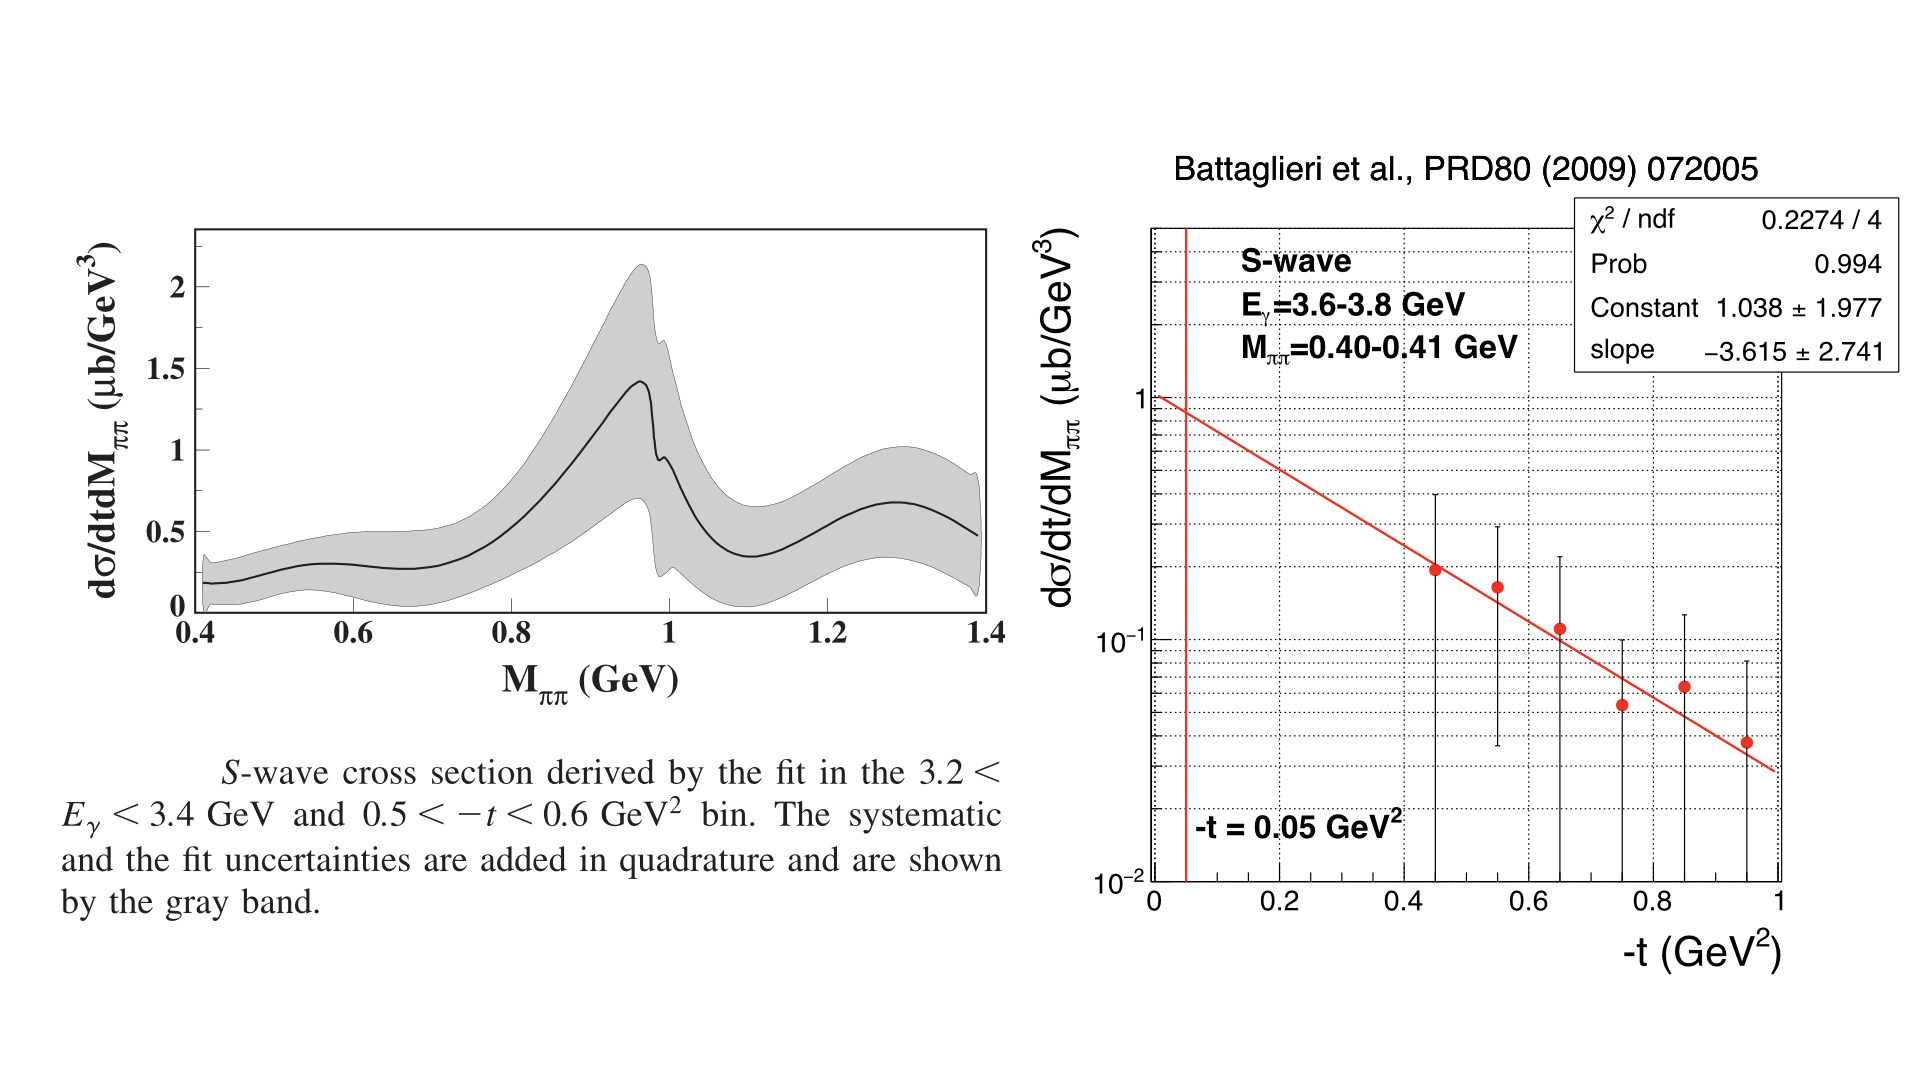
\includegraphics[width=6in]{figures/f0_500.png}
\caption{CLAS data for s-wave $\pi^+ \pi^-$ photoproduction on the proton at $3.2 < E_\gamma < 3.4$ GeV \cite{Battaglieri:2009aa}. }
\label{f0_500}
\end{figure}

\begin{figure}
\centering
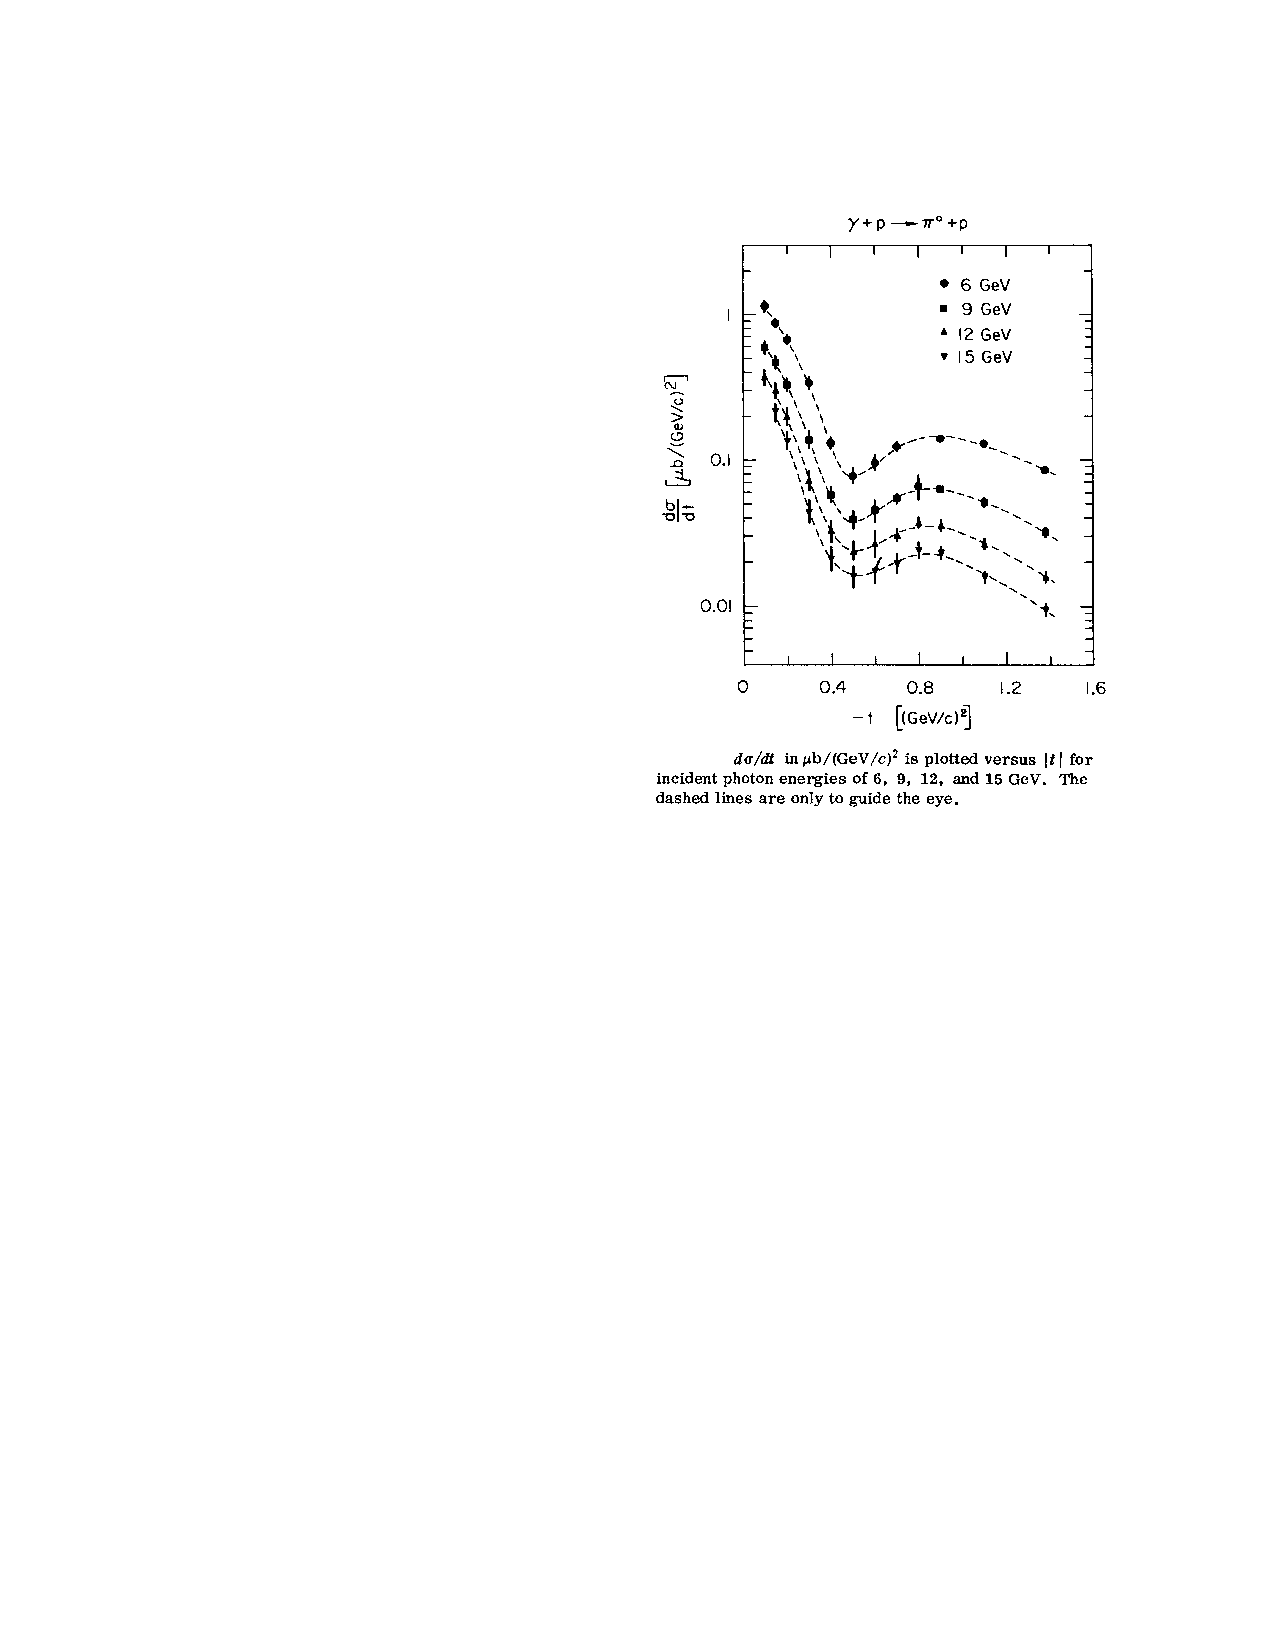
\includegraphics[width=4in]{figures/SLAC_data.pdf}
\caption{SLAC data for $\pi^0$ photo-production on the proton \cite{Anderson:1971}.}
\label{SLAC}
\end{figure}